\chapter{de Sitter 视界与宇宙学概率}

\lectureoverview{视界不仅仅是一个因果边界。对于静止观测者而言，它是一个热系统：在距视界固有距离 \(\rho\) 处放置的温度计读出的温度量级为 \(1/(2\pi\rho)\)，而引力红移使得远处看到的辐射要冷得多。我们将把这一黑洞的经验带入 de Sitter 空间，推导固定的视界半径 \(H^{-1}\)，并写出观测者的静态区度规。讲座的后半部分将追踪热力学的令人不安的后果：有限的 de Sitter 熵、Poincaré 回归、Boltzmann 大脑、永恒暴胀以及测度问题。最后的讨论将弦理论中精确的超对称结构与可能描述我们世界的、仍然未知的框架区分开来。}

\section{视界为何是热的}

我们在正式讲座之前开始，先提出决定今晚方向的问题。

\begin{classroomqa}
\audiencequestion{宇宙视界中并不包含黑洞。那么它究竟通过什么机制可以是热的？\lecturetimestamp{00:00:17}}
\lecturerresponse{机制与黑洞视界相同。有用的问题是操作性的：在视界附近放置的温度计记录到什么，以及什么样的辐射会到达远离视界的观测者？}
\end{classroomqa}

第一个实验是局部的。将温度计保持在距任意光滑、非极端视界的固定固有距离 \(\rho\) 处。足够靠近视界时，几何具有普适的 Rindler 形式，温度计读数为
\begin{equation}
T_{\rm local}(\rho)\simeq \frac{1}{2\pi\rho}
\label{eq:l09-local-temperature}
\end{equation}
其中采用 \(\hbar=c=k_B=1\) 的单位制。恢复常数后得到
\begin{equation}
k_B T_{\rm local}(\rho)\simeq \frac{\hbar c}{2\pi\rho}.
\end{equation}
当 \(\rho\to0\) 时的发散并不意味着下落观测者会遇到一个普通的物质火炉。它是由一位始终静止在视界外侧、因而必须越来越剧烈地加速的观测者所赋予的温度。

开场对话还区分了三个容易被混为一谈的概念：能量、温度和熵。

\begin{classroomqa}
\audiencequestion{如果把光子送入黑洞，我们测量的熵是否仍然相同，还是只有能量发生变化？\lecturetimestamp{00:01:22}}
\lecturerresponse{一旦光子变得不可及、位于视界之后，额外的信息就被隐藏了。在这里使用的简化比特语言中，一个光子可以隐藏一个额外的比特，从而增加熵。能量、温度和熵相互关联，但它们不可互换。}
\end{classroomqa}

\editorialnote{对于物理黑洞，熵变由 \(dS=dE/T_H\) 在热力学上确定；它并非对每个光子都普遍地为一个比特，而与能量无关。一比特的说法是讲座中的信息论理想化。}

近视界区域不断发射并重新吸收高频量子涨落。视界使这些涨落对静止观测者而言成为热性的。然而这立即引出一个谜题。如果该区域任意地热，为什么远处的观测者没有被任意高能的 photon 致盲？

\section{红移与 Hawking 温度}

普通的炽热墙壁即使我们站得很远，仍然是高频辐射的源。视界则不同，因为它的辐射必须爬过引力红移。光子的速度仍为 \(c\)；减小的是它的能量，
\begin{equation}
E=\hbar\omega,
\qquad
\omega_{\rm received}<\omega_{\rm emitted}.
\end{equation}
讲座中使用的粉笔类比仅在此点之前有用。抛出的石头上升时会减速，而光子继续以光速运动，同时其频率和能量减小。

对于 Schwarzschild 黑洞，无穷远处观测者测得的温度为
\begin{equation}
T_H=\frac{1}{8\pi M}
\label{eq:l09-hawking-natural}
\end{equation}
其中单位为 \(G_N=\hbar=c=k_B=1\)。在普通单位中，
\begin{equation}
T_H=\frac{\hbar c^3}{8\pi G_N M k_B}.
\label{eq:l09-hawking-full}
\end{equation}

\begin{figure}[htbp]
\centering
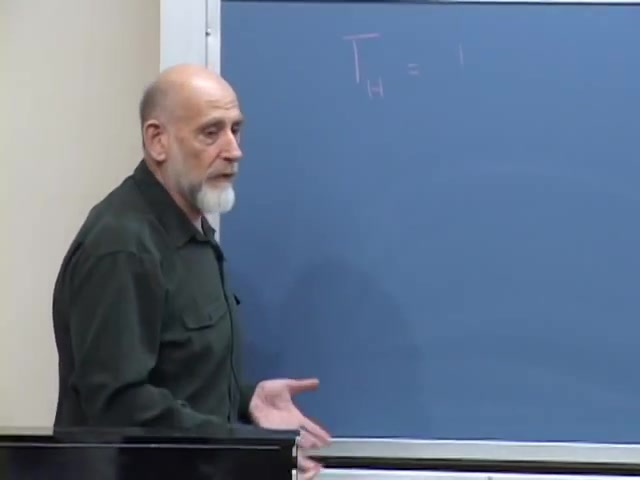
\includegraphics[width=0.68\textwidth]{lecture_09_figure_02.png}
\caption{自然单位下的 Hawking 温度 \(T_H=1/(8\pi M)\)。}
\lectureframe{00:08:12}
\end{figure}

更大的黑洞更冷。讲座通过追溯一个典型光子的反向路径来解释这一点。热光子具有特征能量 \(E_\gamma\sim T_H\)。一个以 \(M^{-1}\) 量级的能量到达无穷远的光子，当它从视界附近出发时具有大得多的局域能量。对于更大的黑洞，近视界层与无穷远之间的红移更为严重，从而留下更低的渐近温度。

\begin{classroomqa}
\audiencequestion{如果 Schwarzschild 时间在视界处冻结，我们是否应该追踪最初落入并构建了黑洞的那个光子？\lecturetimestamp{00:04:19}}
\lecturerresponse{对于温度问题，应追踪向外发射的光子。它们以非常高的局域频率出发，在向外爬升时损失能量，并作为 Hawking 辐射到达。最初下落光子的命运是一个独立的信息问题。}
\end{classroomqa}

\section{Planck 层与拉伸视界}

方程~\eqref{eq:l09-local-temperature}中的局域关系能在多大程度上被信任？本讲将普朗克长度视为半经典描述中有意义的最短距离。这提示存在一个薄层，大致位于数学视界之外一个普朗克长度处，其中充满普朗克尺度的涨落。它持续地发射和吸收。

大多数发射出的量子并不会逃逸。只有那些被导向一个非常狭窄的向外锥体内的量子才能避免落回。以一般角度发射的量子会返回视界。出射和入射的激发相互碰撞，产生粒子对和其他粒子；在这个意义上，定态描述包含一层极热物质的薄壳。

\begin{figure}[htbp]
\centering
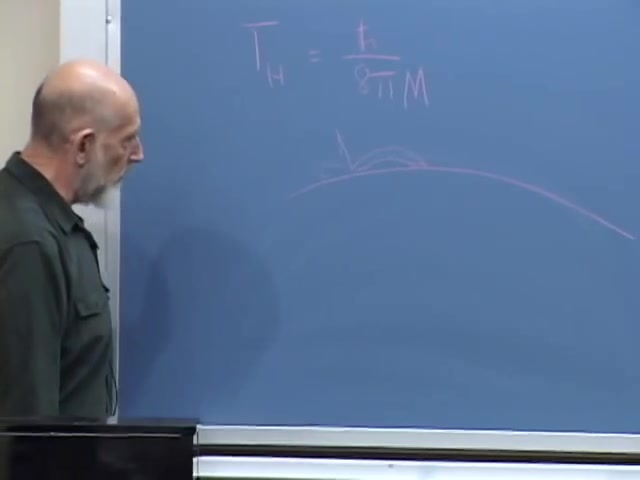
\includegraphics[width=0.74\textwidth]{lecture_09_figure_03.png}
\caption{近视界辐射的狭窄逃逸锥。大多数局域发射的量子返回视界。}
\lectureframe{00:11:38}
\end{figure}

存在一个互补的时空图像。远离视界时，一个虚涨落可以示意性地用一个短闭合圈表示：一个粒子-反粒子激发在能够成为渐近态之前就出现并消失。在视界附近，一个涨落可以跨越因果边界。对外部观察者而言，外侧部分看起来像是由视界发射、随后又被重新吸收的粒子。极小一部分逃逸并成为霍金辐射。

\begin{classroomqa}
\audiencequestion{在外部图中，这样的涨落是否从\(t=-\infty\)延伸到\(t=+\infty\)？\lecturetimestamp{00:15:00}}
\lecturerresponse{精确的经典视界导致那种看似奇异的描述。实际上我们用一个拉伸视界来代替它，即位于外部约一个普朗克长度处的一个类时曲面。于是发射和重新吸收在有限的外部时间中发生。}
\end{classroomqa}

\begin{figure}[htbp]
\centering
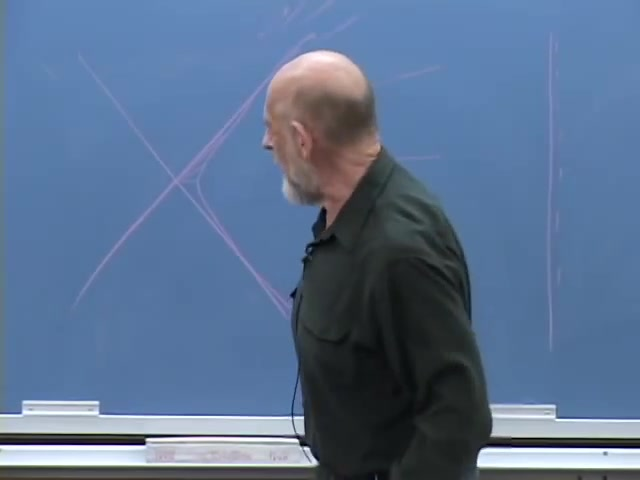
\includegraphics[width=0.72\textwidth]{lecture_09_figure_04.png}
\caption{经典视界以及外部描述中使用的邻近拉伸视界。}
\lectureframe{00:15:52}
\end{figure}

拉伸视界并不是一个新的不变边界。它是一个有效曲面，被放置在半经典几何不再可靠之处。物质以及几何本身的量子涨落将精确位置在普朗克尺度上抹平。这一构造将那种不确定性打包到一个曲面上，使得外部描述在该曲面上仍然有限。

在这个局域论证中，没有任何东西知道视界属于黑洞还是属于加速宇宙。这就是通往德西特空间的桥梁。

\section{膨胀坐标中的德西特空间}

正式讲授从德西特时空的空间平坦切片开始，
\begin{equation}
ds^2=-dt^2+e^{2Ht}d\mathbf{x}^2,
\qquad
d\mathbf{x}^2=dx^2+dy^2+dz^2.
\label{eq:l09-flat-slicing}
\end{equation}
常数\(H\)是德西特膨胀率。因子以\(e^{2Ht}\)的形式出现，是因为度规测量的是距离平方；一个固定的坐标间隔具有物理长度
\begin{equation}
D(t)=e^{Ht}\lvert\Delta\mathbf{x}\rvert.
\end{equation}

\begin{figure}[htbp]
\centering
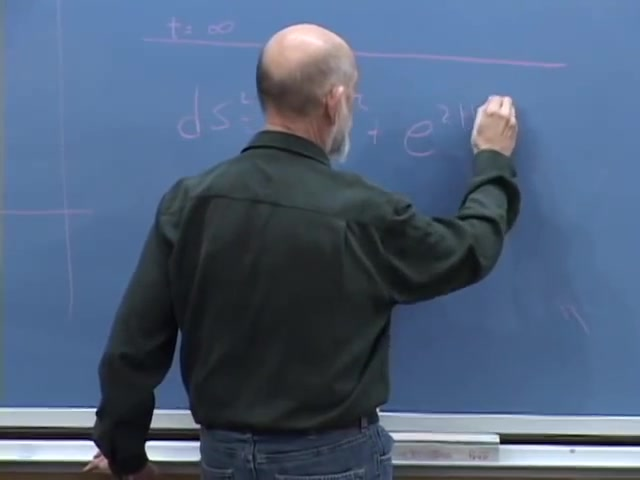
\includegraphics[width=0.78\textwidth]{lecture_09_figure_05.png}
\caption{平坦坐标中指数膨胀的德西特度规。}
\lectureframe{00:18:50}
\end{figure}

这些坐标使膨胀变得透明，但把未来无穷远放在图页上方无穷远处。为了把它带到黑板上，引入共形时间
\begin{equation}
\eta=-\frac{1}{H}e^{-Ht},
\qquad
-\infty<\eta<0.
\label{eq:l09-conformal-time}
\end{equation}
于是
\begin{equation}
dt=\frac{d\eta}{-H\eta},
\qquad
e^{Ht}=-\frac{1}{H\eta},
\end{equation}
而方程~\eqref{eq:l09-flat-slicing}变为
\begin{equation}
ds^2=\frac{1}{H^2\eta^2}
\left(-d\eta^2+d\mathbf{x}^2\right).
\label{eq:l09-conformal-metric}
\end{equation}
当\(t\to+\infty\)时，\(\eta\to0^{-}\)。无限固有时被压缩到有限水平线\(\eta=0\)。

\editorialnote{时间变换在黑板上书写时被修正了数次。方程~\eqref{eq:l09-conformal-time}是一致的形式：早期宇宙时间映射到\(\eta\to-\infty\)，而未来无穷远映射到\(\eta\to0^{-}\)。}

\begin{figure}[htbp]
\centering
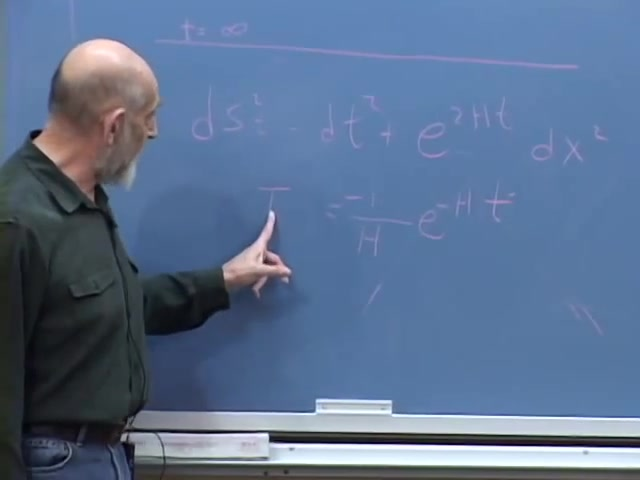
\includegraphics[width=0.82\textwidth]{lecture_09_figure_06.png}
\caption{共形时间变换以及共形平坦度规。}
\lectureframe{00:21:24}
\end{figure}

共形因子同时乘在时间项和空间项上，因此它不改变零方向。对于径向光线，
\begin{equation}
ds^2=0
\quad\Longrightarrow\quad
-d\eta^2+dx^2=0
\quad\Longrightarrow\quad
\frac{dx}{d\eta}=\pm1.
\label{eq:l09-null-rays}
\end{equation}
因此光在共形图中以\(45^\circ\)传播。这就是坐标变换有用的原因：因果可达性变得可见。

\section{一个观察者的因果片区}

想象一个观察者，其世界线延续无限固有时。在紧致化图上，它终止于\(\eta=0\)上的一个点。该观察者能够接收到的每一个信号都位于该终点的后向光锥之内。无论观察者等待多久，锥外的事件都永远无法与该观察者通信。

\begin{figure}[htbp]
\centering
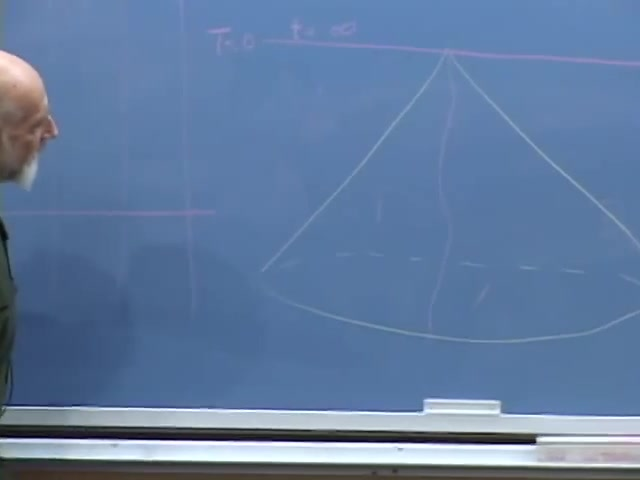
\includegraphics[width=0.78\textwidth]{lecture_09_figure_07.png}
\caption{共形德西特坐标中一个观察者的极限后向光锥。}
\lectureframe{00:24:38}
\end{figure}

第二个观察者有不同的锥。两个可及区域相互重叠，但二者都不是整个时空。在论证的剩余部分，我们采用第一个观察者的视角，并把那个后向光锥称为该观察者的因果片区。

这幅图似乎让这块区域朝未来收缩，但坐标宽度并不是固有距离。在\(\eta\)为常数的切片上，位于\(x=0\)的观测者与位于\(x=\Delta x\)的视界之间的固有距离平方为
\begin{equation}
D^2=\frac{(\Delta x)^2}{H^2\eta^2}.
\label{eq:l09-horizon-distance-start}
\end{equation}
视界是一条\(45^\circ\)的零线，终止于\(\eta=0\)，因此
\begin{equation}
\Delta x=\lvert\eta\rvert.
\end{equation}
代入后得到
\begin{equation}
D_{\rm hor}^2=\frac{1}{H^2},
\qquad
D_{\rm hor}=\frac{1}{H}.
\label{eq:l09-horizon-radius}
\end{equation}
坐标间隔在收缩，但共形因子恰好以补偿的量增长。固有视界半径是常数。

\begin{figure}[htbp]
\centering
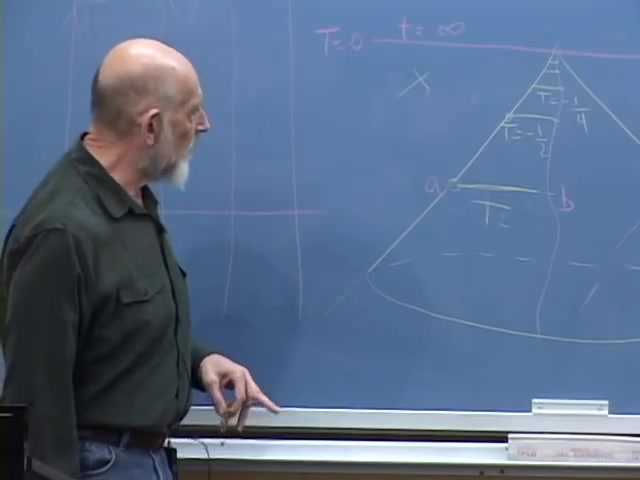
\includegraphics[width=0.80\textwidth]{lecture_09_figure_08.png}
\caption{将收缩的坐标间隔转换为固定固有距离\(H^{-1}\)的黑板推导。}
\lectureframe{00:28:42}
\end{figure}

\section{静态区域}

固定的视界半径提示我们采用适配中心观测者的坐标。讲座没有推导坐标变换，而是直接写出结果：
\begin{equation}
ds^2=
-\left(1-H^2r^2\right)d\tau^2
+\frac{dr^2}{1-H^2r^2}
+r^2d\Omega_2^2.
\label{eq:l09-static-patch}
\end{equation}
系数依赖于\(r\)，而不依赖于\(\tau\)。该图覆盖观测者的静态区域，
\begin{equation}
0\le r<\frac{1}{H}.
\end{equation}

\begin{figure}[htbp]
\centering
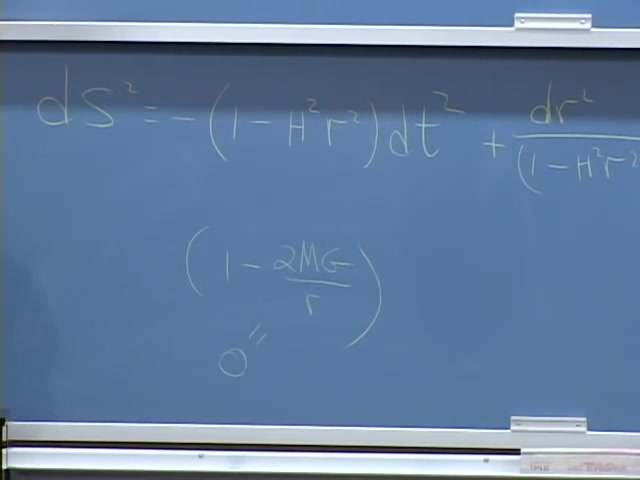
\includegraphics[width=0.88\textwidth]{lecture_09_figure_09.png}
\caption{de Sitter静态区域度规及其与Schwarzschild因子的比较。}
\lectureframe{00:34:22}
\end{figure}

与Schwarzschild的相似性立刻显现：
\begin{equation}
f_{\rm dS}(r)=1-H^2r^2,
\qquad
f_{\rm Schw}(r)=1-\frac{2G_NM}{r}.
\end{equation}
在两种情形中，静态坐标下的视界都出现在\(f(r)=0\)处。对于de Sitter，
\begin{equation}
1-H^2r^2=0
\quad\Longrightarrow\quad
r_H=H^{-1}.
\end{equation}
该图在那里是奇异的，正如Schwarzschild坐标在黑洞视界处奇异一样。然而，整体几何在一个重要方面有所不同。黑洞观测者站在外面向内看；de Sitter观测者站在里面向外看。

\begin{classroomqa}
\audiencequestion{在一个指数膨胀的宇宙中，自由释放的粒子彼此远离，几何怎么可能是静态的？\lecturetimestamp{00:36:06}}
\lecturerresponse{静态并不意味着每个粒子都保持不动。它意味着度规系数以及重复实验的结果与起始时间无关。现在释放两个粒子，它们会加速分离；稍后重复同样的实验，同样的运动仍会发生。}
\end{classroomqa}

\begin{classroomqa}
\audiencequestion{这两个分离的粒子会看到彼此红移吗？\lecturetimestamp{00:38:34}}
\lecturerresponse{会。尽管适配观测者的度规与时间无关，它们不断增大的间距仍会产生相对红移。}
\end{classroomqa}

\section{从内部看到的温度}

Schwarzschild空间与de Sitter空间的近视界结构是局部等价的。因此，de Sitter视界会发射并重新吸收热量子。一个稀有的光子向内传播到中心观测者，在爬升静态区域的势时损失能量。中心测得的Gibbons--Hawking温度为
\begin{equation}
T_{\rm dS}=\frac{H}{2\pi}
\label{eq:l09-de-sitter-temperature}
\end{equation}
（自然单位制）。位于半径\(r\)处的静止温度计读数为Tolman红移后的值
\begin{equation}
T_{\rm local}(r)=
\frac{T_{\rm dS}}{\sqrt{1-H^2r^2}},
\label{eq:l09-tolman}
\end{equation}
当\(r\to H^{-1}\)时它发散，而在视界附近约化为式~\eqref{eq:l09-local-temperature}。

\editorialnote{讲座从视界距离和红移得到标度，而没有明确写出式~\eqref{eq:l09-de-sitter-temperature}和\eqref{eq:l09-tolman}。它们陈述了该论证的标准归一化。}

对于观测到的晚期加速，讲座使用周期估计
\begin{equation}
H^{-1}\sim 20\times10^9\ {\rm light\ years}.
\label{eq:l09-lecture-horizon-estimate}
\end{equation}
于是，一个典型的视界光子具有与数十亿光年相当的波长。这不是微波背景辐射；它要冷得多。

操作性的思想实验是一根宇宙尺度的钓鱼竿。Alice留在\(r=0\)处，把温度计系在一根同时能传输数据的极长线上，并让宇宙排斥把仪器带向外面。她在刚好不到视界处让它停下，等待信号返回，发现局域温度很高。她身旁位于中心的温度计则读出微小的值\(H/(2\pi)\)。同一个视界支持这两种读数，因为它们是在不同的引力势处测得的。

\section{穿越视界}

经典的从外部进行的描述类似于人们熟悉的黑洞故事。位于中心的Bob看着Alice远去。她的信号红移越来越强，到达得越来越慢；她看起来被压扁在视界上，并最终消失。后来的旅行者Jane则表现为边界附近沉积层中的又一层更薄的层。

\begin{classroomqa}
\audiencequestion{从我们的观点看，物体究竟会穿过宇宙视界吗？\lecturetimestamp{00:45:30}}
\lecturerresponse{在静态观测者的经典描述中不会。它们的信号红移并消失，而它们的表观位置趋近视界。然而，在它们自身自由下落的描述中，它们会穿过视界，而不会遇到局部奇异的表面。}
\end{classroomqa}

\begin{classroomqa}
\audiencequestion{视界只对始终留在近旁而不穿越的观测者才是热的吗？自由下落的观测者并不会仅仅因为穿过视界就被烤熟，对吧？\lecturetimestamp{00:48:27}}
\lecturerresponse{艾丽丝在她自己的参考系中平滑地穿过。极端温度属于静止描述。如果鲍勃坚持要把艾丽丝分辨得越来越靠近视界，他就必须用越来越短的波长去照射她。于是，这个尝试中的海森堡显微镜所沉积的能量足以烤熟它试图观测的对象。}
\end{classroomqa}

这并不是两个局域事件之间的矛盾。静止观测者和自由下落者使用的是截然不同的测量。视界互补性所问的是：如何才能使这两种描述都成立，而又不允许一个观测者直接比较重复的信息。

\section{真空排斥的牛顿模型}

此时有学生问，什么取代了黑洞的引力势阱。萨斯坎德通过构造一个牛顿模型来回答。设 \(\phi\) 为引力势，则检验粒子的加速度为
\begin{equation}
\mathbf{a}=-\boldsymbol{\nabla}\phi.
\end{equation}
对于普通的非相对论物质，泊松方程为
\begin{equation}
\nabla^2\phi=4\pi G_N\rho.
\label{eq:l09-poisson}
\end{equation}

\begin{classroomqa}
\audiencequestion{如果黑洞效应来自其引力势阱，那么在德西特空间中相应的源是什么？\lecturetimestamp{00:49:36}}
\lecturerresponse{真空能量本身提供了一个空间上均匀的引力源。在牛顿描述中，它产生的是二次势，而不是 \(1/r\) 势阱。}
\end{classroomqa}

\begin{figure}[htbp]
\centering
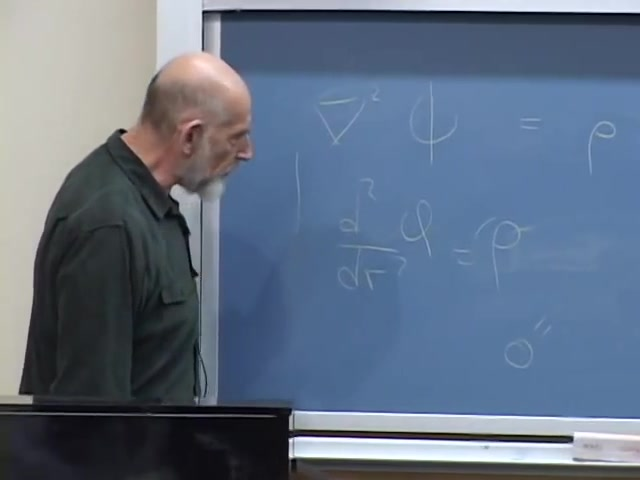
\includegraphics[width=0.78\textwidth]{lecture_09_figure_10.png}
\caption{泊松方程与讲义中示意性的径向二阶导数形式。}
\lectureframe{00:51:38}
\end{figure}

黑板上省略了归一化、球面测度项、压强，起初甚至省略了整体符号，把这个练习简化为
\begin{equation}
\frac{d^2\phi}{dr^2}\sim H^2.
\end{equation}
关键的推断是：常数源给出二次函数。取德西特排斥所需的符号，
\begin{equation}
\phi_{\rm dS}(r)=-\frac{1}{2}H^2r^2,
\qquad
a_r=-\frac{d\phi_{\rm dS}}{dr}=H^2r.
\label{eq:l09-de-sitter-potential}
\end{equation}
加速度指向外侧，并随距离线性增长。解 \(\ddot r=H^2r\) 得到
\begin{equation}
r(\tau)=A e^{H\tau}+B e^{-H\tau},
\end{equation}
因此增长分支再现了指数分离。

\begin{figure}[htbp]
\centering
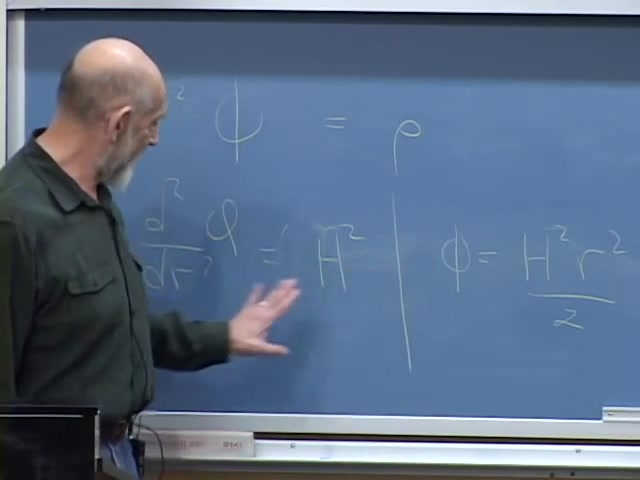
\includegraphics[width=0.76\textwidth]{lecture_09_figure_11.png}
\caption{均匀源方程与二次德西特势。}
\lectureframe{00:53:32}
\end{figure}

\editorialnote{在广义相对论中，均匀流体的弱场加速度取决于 \(\rho+3p\)，而不只是 \(\rho\)。真空能量有 \(p=-\rho\)，所以 \(\rho+3p=-2\rho\)，加速度是排斥性的。式~\eqref{eq:l09-de-sitter-potential} 是正确归一化的德西特结果；黑板上的计算有意只追踪二次依赖关系和符号。}

在中心放置一个普通质量 \(M\)。定性势变为
\begin{equation}
\phi(r)=-\frac{G_NM}{r}-\frac{1}{2}H^2r^2,
\label{eq:l09-combined-potential}
\end{equation}
径向加速度为
\begin{equation}
a_r=-\frac{G_NM}{r^2}+H^2r.
\end{equation}
在小 \(r\) 处，局域吸引占优；在大 \(r\) 处，真空排斥占优。二者的平衡发生在
\begin{equation}
r_\ast=\left(\frac{G_NM}{H^2}\right)^{1/3}.
\label{eq:l09-turnaround}
\end{equation}
这就是讲义中势极大值的干净版本。它定性地解释了为什么邻近的引力束缚系统能够保持在一起，而足够遥远的星系则在加速远离。

\begin{figure}[htbp]
\centering
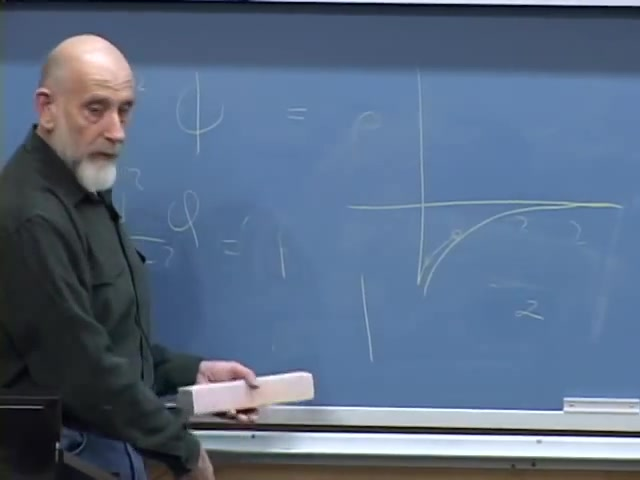
\includegraphics[width=0.78\textwidth]{lecture_09_figure_12.png}
\caption{普通 \(1/r\) 吸引与倒置的二次德西特势相结合。}
\lectureframe{00:58:20}
\end{figure}

\begin{classroomqa}
\audiencequestion{普通力仍然重要吗，还是真空排斥最终会撕碎每一个物质岛屿？\lecturetimestamp{00:57:29}}
\lecturerresponse{必须包括所有力。在足够小的尺度上，电磁束缚和局域引力占主导。真空排斥只有在由 \(H^{-1}\) 以及适合该束缚质量的平衡尺度所设定的巨大距离上才变得重要。}
\end{classroomqa}

\section{一个源，几个名称}

讨论现在在术语上稍作停顿。在所采用的模型中，真空能量、宇宙学常数和暗能量并不是三种相加的物质。它们是同一个 \(w=-1\) 源的三种描述。人们可以谈论爱因斯坦方程中的常数项、真空的洛伦兹不变能量密度，或者驱动晚期加速的分量。

\begin{classroomqa}
\audiencequestion{均匀牛顿源和量子真空能量是否作为两种独立的效应同时存在？\lecturetimestamp{00:59:14}}
\lecturerresponse{不。均匀密度是同一个源的牛顿模型。真空能量、宇宙学常数，以及本讲中的暗能量，指的是同一个物理分量。}
\end{classroomqa}

\begin{classroomqa}
\audiencequestion{那么，同一现象是否既有经典描述又有量子描述？\lecturetimestamp{01:00:32}}
\lecturerresponse{它的微观起源可能是量子力学的，正如电子质量的一部分具有量子起源。一旦有效能量密度已知，它就作为普通源进入经典引力方程。我们并不知道所观测到的值的最终起源。}
\end{classroomqa}

在普朗克单位制中，观测到的真空能量密度极其微小，
\begin{equation}
\rho_\Lambda\sim10^{-123}\rho_{\rm Pl},
\label{eq:l09-planck-smallness}
\end{equation}
这取决于普朗克密度所采用的约定。这个微小的数值就是宇宙学常数问题。这也是视界如此之大的原因：在四维中，
\begin{equation}
H^2=\frac{8\pi G_N}{3}\rho_\Lambda,
\qquad
r_H=H^{-1}.
\end{equation}
如果\(H\)更大，视界就会更小，中心的德西特温度就会更高，排斥性加速度\(H^2r\)就会更强。

\begin{classroomqa}
\audiencequestion{微小的宇宙学常数是否与普朗克常数和量子涨落有关？\lecturetimestamp{01:03:27}}
\lecturerresponse{最清晰的比较使用无量纲的普朗克单位，其中\(G_N=\hbar=c=1\)。在这些单位下，真空密度比自然的普朗克密度低约\(123\)个数量级。解释这一层级结构是基础物理学的核心谜题之一。}
\end{classroomqa}

\begin{classroomqa}
\audiencequestion{真空能量必须是一个严格恒定的宇宙学常数吗？加速组分能否减小并最终趋于零？\lecturetimestamp{01:04:52}}
\lecturerresponse{这在逻辑上是一种可能的替代方案：一个动力学暗能量场可以随时间变化。本讲采用恒定情形，是因为当时可获得的观测越来越倾向于接近宇宙学常数的行为，而不是因为所有替代方案都已被证明不可能。}
\end{classroomqa}

\section{遥远未来的天文学}

在渐近德西特宇宙中，不受引力束缚的结构最终会越过观测者的视界。宇宙微波背景红移到可探测性以下。遥远的星系消失。一位幸存的天文学家可能只看到在一个原本黑暗的区域中一个并合后的局域引力岛。

\begin{classroomqa}
\audiencequestion{没有望远镜，会有人注意到遥远的星系已经消失了吗？\lecturetimestamp{01:06:17}}
\lecturerresponse{大概不会。严重的问题更为深刻：即使拥有先进的仪器，未来的观测者也可能缺乏我们今天借以推断膨胀的遥远示踪物和微波背景。}
\end{classroomqa}

那时，古老的岛宇宙图景可能显得很有说服力。奥伯斯佯谬不会迫使得出不同的结论，因为它假设了无限、静态、均匀的发光源分布；未来的观测者只会看到局域岛中有限的恒星。暗能量并不会不断从空无一物的空间中制造出替代星系。

精确德西特空间中的视界并不会围绕局域星系收缩。它的物理半径保持为\(H^{-1}\)，远大于一个星系。消失的是被带过那个固定因果边界的非束缚物质。

\begin{classroomqa}
\audiencequestion{从星系中抛射出的恒星能否作为检验天体来探测大尺度几何？\lecturetimestamp{01:11:25}}
\lecturerresponse{在一段时间内可以。被抛射的物体和长基线光信号可以探测几何。但只有当距离达到十亿光年的相当一部分量级时，效应才变得显著，因此该实验将需要宇宙学时间尺度。}
\end{classroomqa}

\begin{classroomqa}
\audiencequestion{我们怎么知道一个遥远的视界还没有把宇宙的大部分对我们隐藏起来？\lecturetimestamp{01:11:45}}
\lecturerresponse{我们已经看到足够多的星系、红移和背景辐射，足以测量膨胀并重建大尺度几何。被剥夺了这些示踪物的未来观测者将面临困难得多的推断问题。}
\end{classroomqa}

\begin{classroomqa}
\audiencequestion{如果视界恰好位于仙女座星系之外，它的存在会显而易见吗？\lecturetimestamp{01:12:19}}
\lecturerresponse{会。如此小的视界将要求大得多的\(H\)，由此产生的排斥将强烈改变仙女座星系（Andromeda）的运动。而测量值反而把渐近视界置于一个大得多的尺度上。}
\end{classroomqa}

\begin{classroomqa}
\audiencequestion{在我们的视界之外，是否可能正在发生新的大爆炸？\lecturetimestamp{01:13:25}}
\lecturerresponse{视界之外的事件对我们或我们的后代都不可见。一个相关但更精确的可能性，即永恒暴胀中的气泡成核，将在本讲后面介绍。}
\end{classroomqa}

借助火箭、时钟以及数十亿年的时间，未来的观测者可以派遣探索者穿越这片区域的大部分，并重建其度规。然而，在普通的实验室或文明时间尺度上，这一效应几乎无法触及。这一区分纠正了那个过强的断言，即膨胀将不可能被发现：它在操作上遥不可及，但并非原则上被禁止。

\begin{classroomqa}
\audiencequestion{未来的探索者能否比等待热复现更早得多地确定几何？\lecturetimestamp{01:21:40}}
\lecturerresponse{当然可以。复现并不是所提议的测量。探索者在数十亿光年的基线上交换光信号，可以在短得多、但仍属宇宙学的时间尺度上绘制静态区域。}
\end{classroomqa}

\begin{classroomqa}
\audiencequestion{红移会抹去这类探索者返回的所有信息吗？\lecturetimestamp{01:23:24}}
\lecturerresponse{如果他们在远处于视界内部的尺度上探测，就不会。约十亿光年的基线已经对膨胀敏感，同时只产生适度的红移。该实验主要受限于其极其漫长的持续时间。}
\end{classroomqa}

\section{有限熵与复现}

静态区域在热力学意义上并非空无一物。其视界具有面积
\begin{equation}
A_H=4\pi H^{-2},
\end{equation}
温度 \(T_{\rm dS}=H/(2\pi)\)，以及熵
\begin{equation}
S_{\rm dS}=\frac{A_H}{4G_N}
=\frac{\pi}{G_NH^2}
\label{eq:l09-de-sitter-entropy}
\end{equation}
单位为 \(\hbar=c=k_B=1\)。该熵是有限的。因此，人们可以谨慎地将静态区域描绘为一个有限熵的热腔，在稳态描述中其激发集中在视界附近。

处于平衡态的普通气体盒子在短时间尺度上看起来毫无特征，但统计力学并不禁止涨落。如果一个宏观态相对于平衡态具有熵亏 \(\Delta S\)，其概率大致为
\begin{equation}
P\sim e^{-\Delta S}.
\label{eq:l09-fluctuation-probability}
\end{equation}
相应的等待时间按如下方式增长
\begin{equation}
t\sim t_0 e^{\Delta S}.
\end{equation}
对于有限系统，重新访问一个任意接近先前状态的状态所需的时间就是庞加莱复现时间，
\begin{equation}
t_{\rm rec}\sim H^{-1}e^{S_{\rm dS}}.
\label{eq:l09-recurrence}
\end{equation}
由于我们视界的 \(S_{\rm dS}\) 约为 \(10^{120}\) 量级，讲座将该尺度概括为 \(e^{10^{120}}\)。前因子是以年、哈勃时间还是微观单位来衡量，与双指数相比都无关紧要。

\begin{figure}[htbp]
\centering
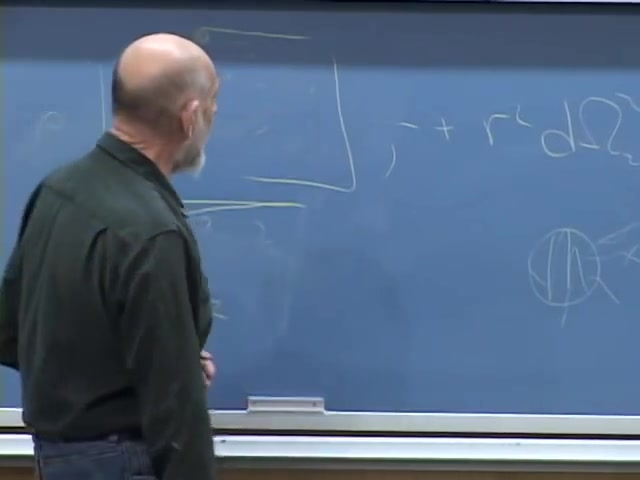
\includegraphics[width=0.76\textwidth]{lecture_09_figure_13.png}
\caption{关于复现的讨论，黑板上写着巨大的指数等待时间尺度。}
\lectureframe{01:16:24}
\end{figure}

在这样的复现之前，较小的涨落要常见得多。房间里的分子可能全部聚集在一个角落；一个复杂的涡旋可能短暂形成；在讲座诙谐的层级中，热运动可能组装出一头大象。所需的熵亏越小，涨落的代价就越低。

\begin{classroomqa}
\audiencequestion{庞加莱复现是否特指量子力学的结果？\lecturetimestamp{01:25:44}}
\lecturerresponse{不是。复现和稀有涨落已经在经典统计力学中出现。将它们应用于德西特空间使用的是我们目前的物理框架，这一框架有朝一日可能被修正，但热力学和统计推理是我们所知最稳固的结构之一。}
\end{classroomqa}

概率本身的含义可能在未来理论中加深。萨斯坎德并未声称相反。他更狭义的观点是，仅仅因为统计力学的长期含义显得奇怪就抛弃它，将丢弃物理学中经过最充分检验的组织原则之一。

\section{玻尔兹曼大脑与典型观测者}

假设一次热涨落创造出一个完整的类大爆炸状态。那需要巨大的熵减少。产生一个太阳系的涨落代价更低；一个已经温暖的 Earth 代价还要更低。如果唯一的要求是一个观测者，那么代价最低的涨落可能只创造出一个功能完备的大脑，并带有看似真实的记忆。这样一个假想的观测者被称为玻尔兹曼大脑。

问题不在于某一次奇异的涨落在逻辑上是否可能。而在于一个宇宙学模型是否预言几乎每一个观测者都是这样的涨落。我们从观测出发进行推理时，假设我们并非极其非典型。如果一个理论中具有连贯宇宙历史的普通观测者被孤立的熱大脑以指数方式超过，那就削弱了这一推断。

因此，玻尔兹曼大脑问题命名了一个定量一致性检验。人们将普通观测者的预期丰度与涨落产生的观测者的丰度进行比较。如果后者占主导，那么要么真空必须在它们增殖之前衰变，要么必须改变测度，要么必须重新考虑宇宙学假设。

先前关于紫外--红外联系的问题被明确推迟。复现论证并不依赖于解决那个单独的问题。

\section{永恒暴胀与气泡宇宙}

接下来，讲座在不试图给出完整推导的情况下引入第二个概率问题。一个亚稳态的德西特真空可以成核出一个气泡，其中真空能更低。气泡壁不断膨胀，其内部可以演化成一个开放的弗里德曼--罗伯逊--沃克宇宙。与此同时，周围暴胀的区域继续膨胀并成核出更多的气泡。

\begin{figure}[htbp]
\centering
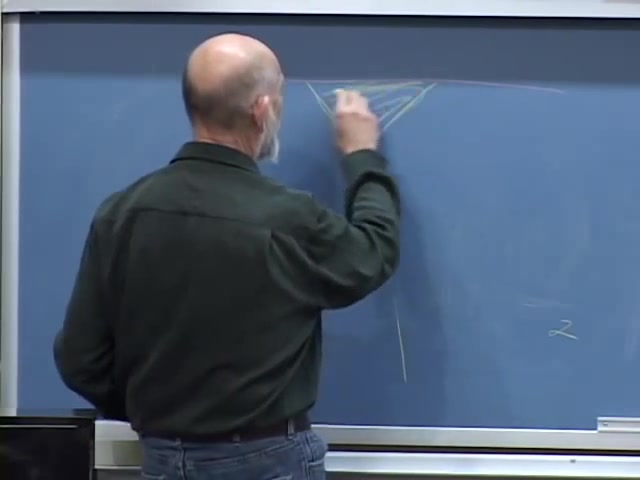
\includegraphics[width=0.74\textwidth]{lecture_09_figure_14.png}
\caption{一个真空能较低的气泡被画在暴胀的德西特背景之中。}
\lectureframe{01:29:38}
\end{figure}

关键特征是种群的指数增长。新物理体积产生的速度比气泡移除它的速度更快，因此气泡区域的数目无界增长。不同的气泡可能落入不同的低能态，从而表现出不同的有效物理。

为了揭示其中的统计困难，萨斯坎德首先离开宇宙学，考虑一个以指数增长、资源有限但未知的人类种群。假设观测者在所有曾经生活过的人中是典型的。如果种群每一代翻一番然后终结，那么一半的人生活在最后一代，四分之三生活在最后两代，八分之七生活在最后三代：
\begin{equation}
f_n=1-2^{-n}.
\label{eq:l09-last-generations}
\end{equation}
典型性于是会把我们置于令人不安地接近终结的位置，尽管我们对资源总量一无所知。这并不是作为对人类灭绝的可靠预言而提出的。它是一个警告：指数增长使得计数被截断所主导。

抛硬币的例子更清晰地陈述了通常的典型性假设。如果许多实验者每人抛一枚公平的硬币\(N\)次，绝大多数人会得到
\begin{equation}
n_H=\frac{N}{2}+O(\sqrt{N}).
\end{equation}
一个极端的观测者应当首先怀疑模型有误或硬币有问题，而不是在没有证据的情况下假定自己处于一个极其罕见的尾部。宇宙学概率使用同样的典型性直觉，但在无限种群中，它需要一种定义良好的计数方式。

\section{埃舍尔的边界与测度问题}

萨斯坎德的几何类比是M.\ C.\ 埃舍尔的\emph{圆极限IV}，即那个由天使与魔鬼铺满、越靠近边界显得越小的圆盘。在图画所表示的双曲几何中，这些图形是等价的；它们表观的欧几里得大小发生变化，仅仅是由于投影。

\begin{figure}[htbp]
\centering
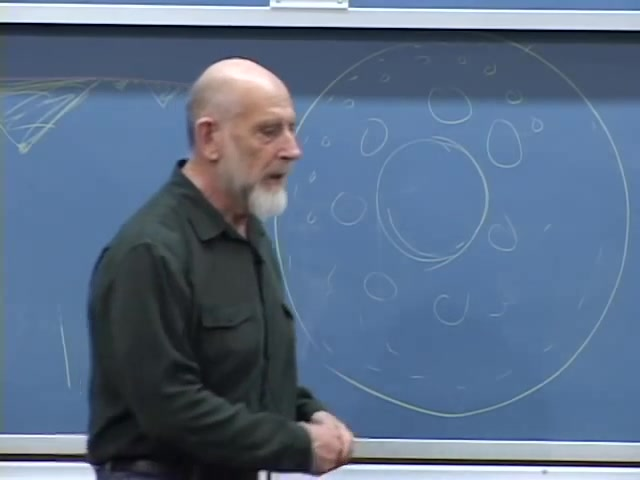
\includegraphics[width=0.76\textwidth]{lecture_09_figure_15.png}
\caption{埃舍尔在圆形边界附近指数增殖的图形在黑板上的替代物。}
\lectureframe{01:37:54}
\end{figure}

设想埃舍尔只有有限的时间、墨水和耐心。在边缘附近他最终会停下来，也许留下一些未完成的图形。由于图形数目随双曲半径指数增长，一个有限的外层包含所画每一个图形的一个固定比例。无论把截断向外移动多远，大致一半都可以位于最后一层中。

现在问天使与魔鬼之比。在理想的无限图案中，对称性暗示二者一一相等。然而在任何有限的计数中，一个稍有不同的边界都可能包含多得多的某一类图形。由于计数的大部分位于边界附近，该边界的微小形变就会使答案产生量级为一的变化。

\begin{figure}[htbp]
\centering
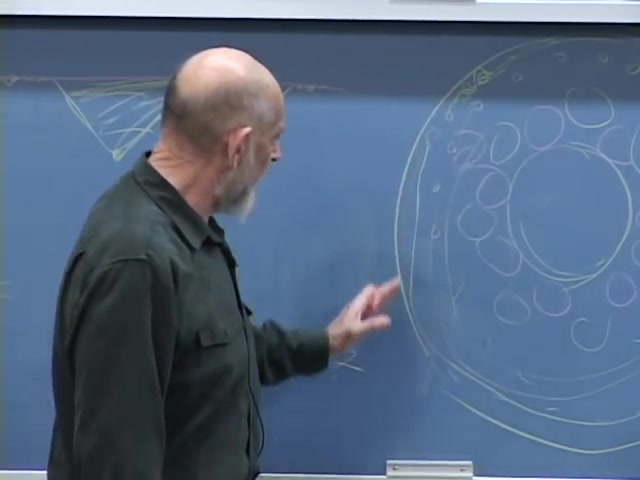
\includegraphics[width=0.76\textwidth]{lecture_09_figure_16.png}
\caption{在指数增长的图案中，截断边界主导着计数。}
\lectureframe{01:43:06}
\end{figure}

同样的模糊性出现在永恒暴胀中。数出某个时间截断以下的蓝色和粉色气泡宇宙，然后把截断推后。两种计数都发散，而它们的比值可能敏感地依赖于\emph{时间}意味着什么以及截断曲面如何画出。概率测度是一种对无限种群进行正规化并提取相对概率的规定。不同的看似合理的规定无法彼此一致，这就是测度问题。

\begin{classroomqa}
\audiencequestion{这个截断问题与重整化之间有关系吗？\lecturetimestamp{01:45:43}}
\lecturerresponse{有一个类比。在量子场论中，人们引入点阵或紫外截断，将其细化，并寻求对正规化子边缘细节不敏感的物理量。宇宙学家希望从永恒暴胀中得到同样稳健的提取，但在本文所讨论的框架中，目前还没有同样决定性的规定可用。}
\end{classroomqa}

这个类比不应被夸大。当受控的流确定出与正规化子无关的可观测量时，重整化才成功。测度问题恰恰在于，类似的不变量问题和取极限的程序仍然不清楚。说我们也许问错了问题，在给出正确的问题之前并不是一个解决方案。

\begin{classroomqa}
\audiencequestion{这个气泡图像与早期宇宙中的暴胀是同一种现象吗？\lecturetimestamp{01:48:19}}
\lecturerresponse{二者密切相关。在永恒暴胀中，母背景继续暴胀，而局部气泡内部则经历各自的宇宙学演化。我们的可观测宇宙可能位于这样一个区域之内。}
\end{classroomqa}

\section{气泡碰撞能被观测到吗？}

两个气泡相遇时，并不是简单地把它们的真空能相加。一个畴壁将真空态不同的区域分隔开来，而畴壁的几何形状决定了任一侧能够观测到什么。取决于碰撞相对于我们过去光锥的位置，其印记可能被隐藏，也可能可见。

\begin{classroomqa}
\audiencequestion{两个真空气泡碰撞时会发生什么？\lecturetimestamp{01:52:07}}
\lecturerresponse{碰撞会产生一种畴壁几何，其行为取决于两个真空以及壁的张力。在有利的因果条件下，这种扰动可以进入我们的可观测区域，并留下各向异性的印记。}
\end{classroomqa}

讲座讨论了宇宙微波背景中的一个冷斑区域作为可能的候选，并指出圆形特征周围的偏振可作为判别依据。这是有意作为一种可能性提出的，而非一项探测结果。一个有说服力的碰撞印记将是革命性的，因为它将为邻近气泡区域提供直接证据，并使测度问题在实验上变得紧迫。

\begin{figure}[htbp]
\centering
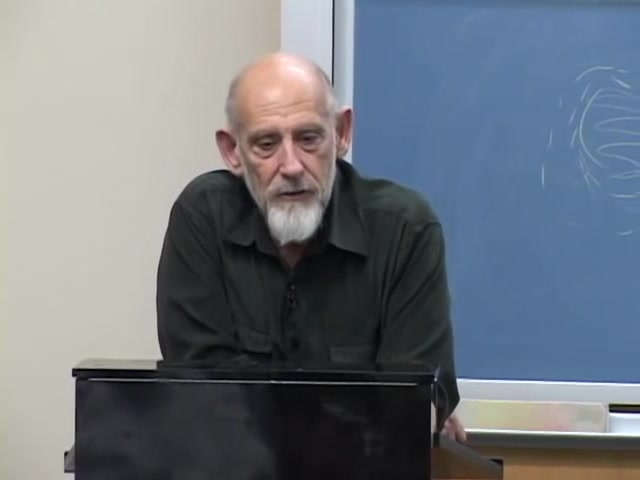
\includegraphics[width=0.70\textwidth]{lecture_09_figure_17.png}
\caption{气泡碰撞讨论中的圆形天空特征及其可能的偏振图样。}
\lectureframe{01:50:22}
\end{figure}

\editorialnote{冷斑的讨论记录了讲座当时的观测状况和提议。仅凭一个温度异常并不构成气泡碰撞的证据；还需要一个详细的、相互关联的印记。}

\begin{classroomqa}
\audiencequestion{这些气泡是四维的吗？其内部具有什么样的空间曲率？\lecturetimestamp{01:53:37}}
\lecturerresponse{它们是时空区域，而不是在外部时间中演化的三维肥皂泡。其内部通常是具有负空间曲率的开放FRW宇宙。碰撞会扰动该几何，但并不会简单地把负曲率变成正曲率。}
\end{classroomqa}

\section{弦理论确立了与未确立什么}

最后的讨论以邀请听众为弦理论正确赋予一个概率开始。Susskind拒绝给出这个数字，因为该命题过于含糊。他转而区分两个主张。

第一，存在一个高度受约束的、结合了量子力学与引力的数学结构。它产生了精确的结果和深刻的数学恒等式，其内部自洽性经受住了广泛的审视。用讲座中的非正式说法，这就是大写的\emph{String Theory}，即\(S\)。被理解得最清晰的那些版本严重依赖于超对称。

第二，观测到的世界在可及能量上并不是超对称的。要把精确的超对称构造与我们这个非超对称的宇宙联系起来，需要超对称破缺以及一个无法以同等精度加以控制的更大框架。用讲座中的说法，那个被寄予希望的扩展就是小写的\emph{string theory}，即\(s\)。

\begin{classroomqa}
\audiencequestion{人们能否为弦理论是自然的正确理论赋予一个概率？\lecturetimestamp{01:54:18}}
\lecturerresponse{如果不指明指的是哪一个主张，就无法负责任地做到。精确的数学结构确实存在，并且包含量子引力，但严格受控的超对称模型并不是字面意义上的我们所观测到的世界。一个更大的扩展是否包含我们的世界，是物理学家可以持有有根据的偏见的问题，而不是一个定义明确的数值概率。}
\end{classroomqa}

这里可以类比于完整数学工具尚未出现之前的力学。人们可能知道\(F=ma\)和平方反比力，却只能求解高度对称的圆轨道。可求解的部分会是真实的，但并不是整个理论。同样，精确的超对称弦构造可能只是一个更大结构中的一个特殊的、异常易于处理的区域。

\begin{figure}[htbp]
\centering
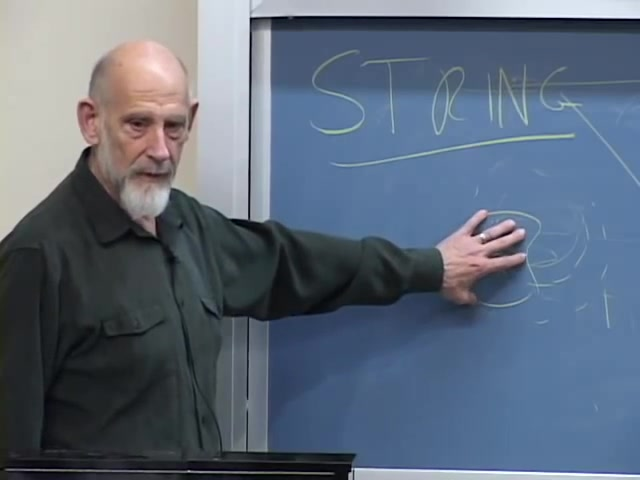
\includegraphics[width=0.60\textwidth]{lecture_09_figure_18.png}
\caption{讲座中的嵌套图景：严格受控的超对称弦构造位于一个推测上更大的框架之内。}
\lectureframe{01:57:34}
\end{figure}

\begin{classroomqa}
\audiencequestion{为什么不直接在精确理论中破缺超对称？\lecturetimestamp{01:57:02}}
\lecturerresponse{许多近似构造研究超对称破缺，但恰恰缺少的是完全可控的非超对称骨架。人们可以在作出标准近似之后进行计算，却并不总是知道这些近似所趋近的精确对象是什么。}
\end{classroomqa}

\begin{classroomqa}
\audiencequestion{精确的超对称理论是否排除了一个包含我们世界的更大、对称性更低的扩展？\lecturetimestamp{02:00:33}}
\lecturerresponse{不。它确立的是，观测到的世界并非仅由精确的超对称部分描述。它既未证明也未否证这一部分与一个包含现实物理的更大理论相关联。}
\end{classroomqa}

\begin{classroomqa}
\audiencequestion{弦构造是否包含类似于粒子物理对称性破缺的对称性破缺？\lecturetimestamp{02:01:21}}
\lecturerresponse{关于超对称破缺已有大量工作，对超对称数学也已有许多了解。尚未解决之处在于一个精确的非微扰表述，它将现实的破缺与完整理论结合起来，而不仅仅与可控近似结合起来。}
\end{classroomqa}

\begin{classroomqa}
\audiencequestion{狭义相对论在弦理论中是作为假设，还是作为预言而出现？\lecturetimestamp{02:03:02}}
\lecturerresponse{底层规则是洛伦兹不变的，尽管一个充满物质的特定背景可以选出一个优先的静止参考系。引力则更加不可避免：弦谱包含一个无质量自旋为二的激发态，其相互作用与引力子相同。}
\end{classroomqa}

\begin{classroomqa}
\audiencequestion{弦理论与广义相对论及背景无关性是否相容？\lecturetimestamp{02:04:11}}
\lecturerresponse{其低能引力动力学与广义相对论相容，并且局部背景可以被动力学地改变。微妙之处在于渐近边界条件：它们标记了问题本身，并且一般不能通过该时空内的局部操作来改变。}
\end{classroomqa}

讲座以稳健的数学核心与尚未完成的物理外推之间的这一区分作结。这并不是断言该核心无用，也不是声称该外推已经确立。它陈述的是精确知识止于何处。
